\documentclass[12pt, twoside]{article}
\usepackage[letterpaper, margin=1in, headsep=0.2in]{geometry}
\setlength{\headheight}{0.6in}
%\usepackage[english]{babel}
\usepackage[utf8]{inputenc}
\usepackage{microtype}
\usepackage{amsmath}
\usepackage{amssymb}
%\usepackage{amsfonts}
\usepackage{siunitx} %units in math. eg 20\milli\meter
\usepackage{yhmath} % for arcs, overparenth command
\usepackage{tikz} %graphics
\usetikzlibrary{quotes, angles}
\usepackage{graphicx} %consider setting \graphicspath{{images/}}
\usepackage{parskip} %no paragraph indent
\usepackage{enumitem}
\usepackage{multicol}
\usepackage{venndiagram}

\usepackage{fancyhdr}
\pagestyle{fancy}
\fancyhf{}
\renewcommand{\headrulewidth}{0pt} % disable the underline of the header
\raggedbottom
\hfuzz=2mm %suppresses overfull box warnings

\usepackage{hyperref}

\fancyhead[LE]{\thepage}
\fancyhead[RO]{\thepage \\ Name: \hspace{4cm} \,\\}
\fancyhead[LO]{BECA / Dr. Huson / Geometry\\*  Unit 8: Congruence transformations\\* 10 January 2023}

\begin{document}

\subsubsection*{8.6 Homework: Mixed congruence transformations \hfill CCSS.HSG.CO.A.5}
\begin{enumerate}
\item Do Now: Slide $\triangle ABC$ to the right three and up four. Label the image $\triangle A'B'C'$.
\begin{center}
    \begin{tikzpicture}[scale=.55]
    \draw [help lines] (-7,-4) grid (10,6);
    \draw [thick, <->] (-7.4,0) -- (10.4,0) node [right] {$x$};
    \draw [thick, <->] (0,-4.4)--(0,6.4) node [above] {$y$};  
    \draw [thick]
      (-1,-1) node[below left] {$A$}--
      (5,-2) node[below] {$B$}--
      (2,1) node[above right] {$C$}--cycle;  
  \end{tikzpicture}
\end{center}

\item A vector from the origin $\overrightarrow{OA}$ is shown rotated counterclockwise around $O$.
      \begin{enumerate}
        \item Using a protractor, measure the angle of rotation
        \item Mark and label the point $B(3,-4)$. Draw $\overrightarrow{OB}$.
        \item Find the measure of the combined angle, $m\angle A'OB$.
      \end{enumerate}
      \begin{center}
      \begin{tikzpicture}[scale=1]
      \draw [help lines] (-5,-5) grid (5,5);
      \draw [<->] (-5.4,0) -- (5.4,0) node [right] {$x$};
      \draw [thick, <->] (0,-5.4)--(0,5.4) node [above] {$y$};
      \foreach \x in {-5,...,-1,1,2,3,4,5}
        \draw[shift={(\x,0)},color=black] (0pt,-3pt) -- (0pt,3pt) node[below=5pt]  {$\x$};
      \foreach \y in {-5,...,-1,1,2,3,4,5}
        \draw[shift={(0,\y)},color=black] (-3pt,0pt) -- (3pt,0pt) node[left=5pt]  {$\y$};
        \draw [dashed] (0,0) circle [radius=5cm];
        \draw [line width=2pt, ->] (0,0)--(5,0) node [above left] {$A$};
        \draw [line width=2pt, ->] (0,0)--(4,3) node [above right] {$A'$};
    \end{tikzpicture}
  \end{center}

\newpage


  \item In the diagram below, $\triangle ABC$ with sides of 13, 15, and 16, is mapped onto $\triangle DEF$ after a clockwise rotation of $90^\circ$ about point $P$. 
  \begin{multicols}{2}
    \begin{enumerate}
      \item What is $A$ mapped to? $A \rightarrow$ \vspace{1.5cm}
      \item What corresponds to $F$? \vspace{1.5cm}
      \item Given $DF=3x+1$. Find $x$. \vspace{1.5cm}
    \end{enumerate}
    \begin{tikzpicture}[scale=.6, rotate=-30]
      %\draw [thick, <->] (-7.4,0) -- (10.4,0) node [right] {$x$};
      %draw [thick, <->] (0,-5.4)--(0,10.4) node [above] {$y$};
      \fill (0,0) circle[radius=0.1] node[right]{$P$};
      \draw [thick]
        (-2,1) node[below left] {$A$}--
        (-7,2) node[left] {$B$}--
        (-4,5) node[above right] {$C$}--cycle;
        \node at (-5,1.5)[below]{16};
        \node at (-6,4){13};
        \node at (-2.5,3.5){15};
        \node at (3.25,2.25){$3x+1$};
      \draw [thick]
        (1,2) node[left] {$D$}--
        (2,7) node[above] {$E$}--
        (5,4) node[right] {$F$}--cycle;
    \end{tikzpicture}
  \end{multicols}
  \vspace{2cm}

\newpage
\item On the axes below, graph the point $P(2,4)$ and its image, $P'$, after a rotation of $90^\circ$ counterclockwise around the origin. Label both points as a coordinate pair.
    \begin{center}
      \begin{tikzpicture}[scale=.7]
      \draw [help lines] (-5,-5) grid (5,5);
      \draw [thick, <->] (-5.4,0) -- (5.4,0) node [right] {$x$};
      \draw [thick, <->] (0,-5.4)--(0,5.4) node [above] {$y$};
      \foreach \x in {-5,...,-1,1,2,3,4,5}
        \draw[shift={(\x,0)},color=black] (0pt,-3pt) -- (0pt,3pt) node[below=5pt]  {$\x$};
      \foreach \y in {-5,...,-1,1,2,3,4,5}
        \draw[shift={(0,\y)},color=black] (-3pt,0pt) -- (3pt,0pt) node[left=5pt]  {$\y$}; 
    \end{tikzpicture}
  \end{center}

\end{enumerate}
\end{document}
